\section{Modelagem e Definições Técnicas}

Nesse tópicos, serão abordados os diagramas e modelagens necessários para o desenvolvimento do projeto Lixt. Além disso, serão apresentadas as definições técnicas necessárias para o prosseguimento do projeto.

\subsection{Modelo Entidade-Relacionamento (MER)}

O Modelo Entidade-Relacionamento (MER) é a primeira abstração do banco de dados, no qual é modelado e estruturado a forma no qual os dados serão trabalhados, persistidos e buscados.

\subsubsection{Padrões de Banco de Dados}

Antes de tudo, é necessário definir os padrões utilizados para definir o banco de dados. O banco de dados foi modelado em inglês com o intuito de apresentar coerência com o desenvolvimento.

Todas as tabelas começam o prefixo ``tb\_''. Exemplo: tb\_usuario. Todas as colunas possuem o prefixo de seu tipo:

\begin{itemize}
	\item \underline{Chaves Primárias e Estrangeiras}: Começam com ``id\_''. Exemplo: id\_user.
	\item \underline{Dados de Texto}: Começam com ``st\_'', de string. Exemplo: st\_name.
	\item \underline{Dados Numéricos}: Começam com ``dt\_'', de date. Exemplo: dt\_createdAt.
	\item \underline{Dados de Texto}: Começam com ``nr\_'', de number. Exemplo: nr\_price.  
	\item \underline{Enum}: Começam com ``en\_'', sendo que os enums serão tratados no backend. Exemplo: en\_status.  
\end{itemize}

Quanto aos índices e restrições, é definido o uso dos seguintes prefixos precedidos pelo nome da tabela:

\begin{itemize}
	\item \underline{Chave Estrangeira}: Começam com ``fk\_''. Exemplo: fk\_listMembers\_user. 
	\item \underline{Unique}: Começam com ``un\_''. Exemplo: uq\_user\_email.
	\item \underline{Outros Índices}: Começam com ``idx\_''. Exemplo: idx\_user\_name. 
\end{itemize}


\subsubsection{Apresentação do MER}

Na \autoref{fig:mer} está explicitado o MER proposto para a aplicação Lixt, sendo um diagrama normalizado e com as boas práticas aplicadas.

\begin{figure}[H]
  \centering
  \caption{Modelo Entidade-Relacionamento}
  \label{fig:mer}
  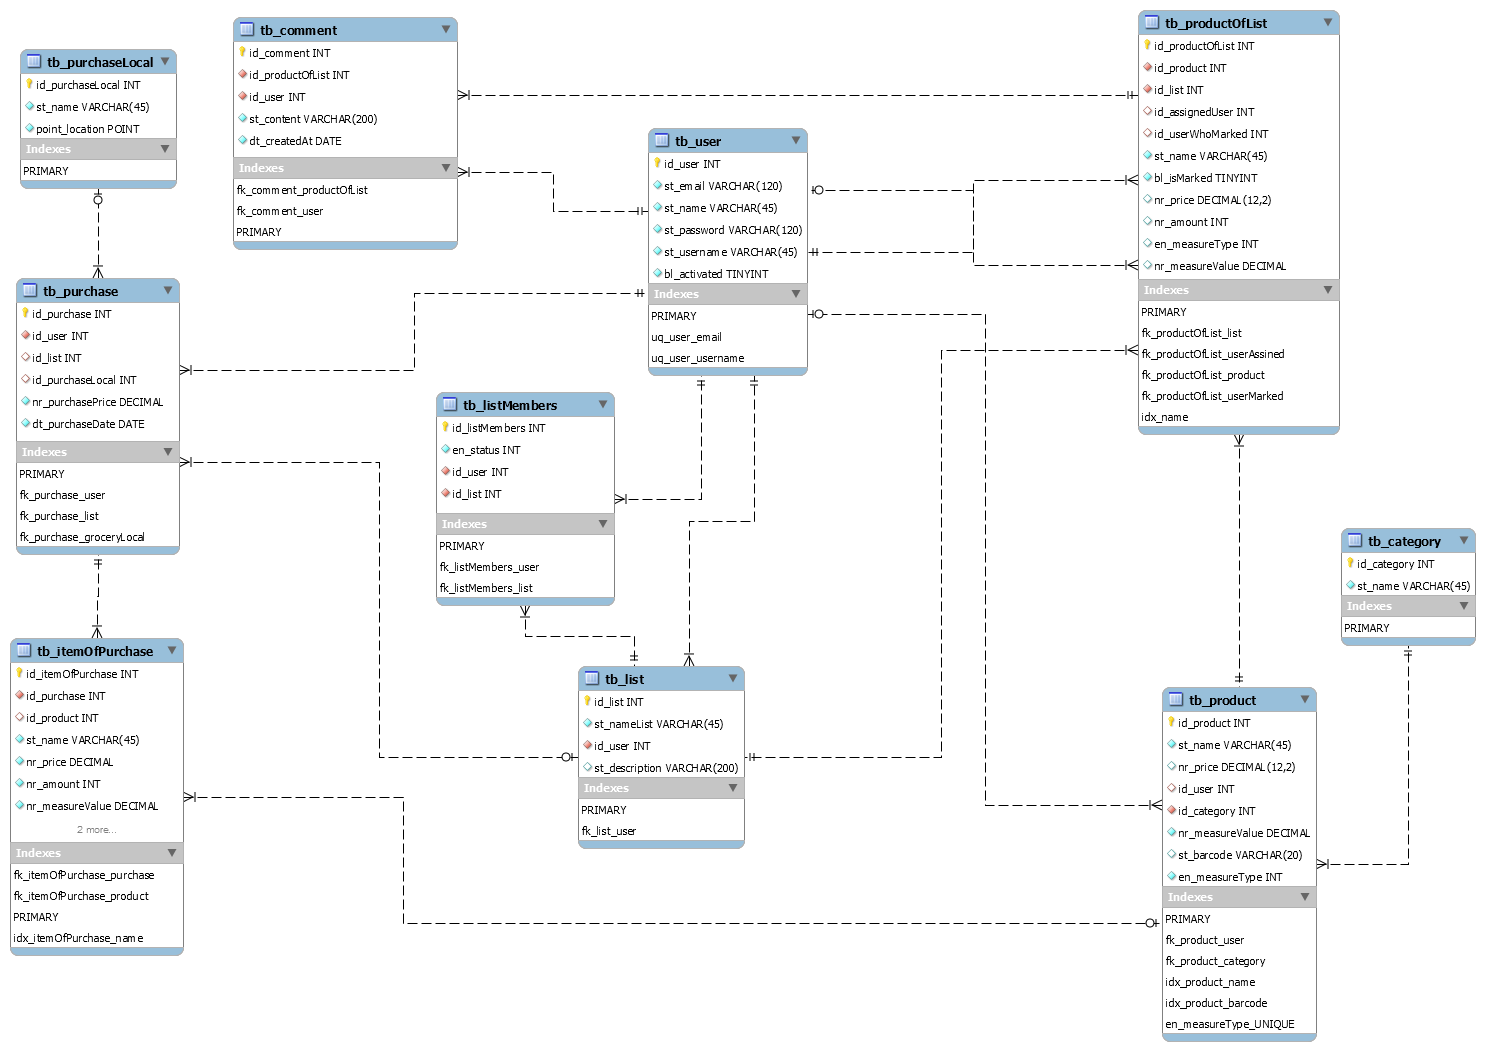
\includegraphics[scale=0.3]{mer}
  \legend{Fonte: Os autores}
\end{figure}

No diagrama, uma lista (tb\_list) possui vários usuário (tb\_user), e um usuário pode estar em várias listas, surgindo assim a necessidade da tabela intermediária (tb\_listMembers). Essa tabela intermediária possui um status, que pode ser ``Aceitado'', ``Rejeitado'' e ``Aguardando Confirmação''.

Um usuário pode fazer vários comentários (tb\_comment) no produto da lista (tb\_productOnList), e um comentário é de um usuário.

Uma lista pode ter várias compras (tb\_purchase), pois uma lista pode ser feita ao decorrer de várias compras, onde uma compra é de um mercado (tb\_purchaseLocal) e possui vários items (tb\_itemOfPurchase).

Tanto um produto da lista quanto um item da compra é 
composto um produto (tb\_product, sendo produto uma tabela mais genérica, pois assim será possível gerar dados estatísticos de produtos mais genéricos sem nenhuma especificidade como, por exemplo, marca do produto), sendo que o produto pode ter uma categoria (tb\_category).

\subsubsection{Definição de Índices}

No MySQL, temos dois tipos de índices:

\begin{enumerate}
	\item \underline{Índice Primário}: Criado pelo MySQL automaticamente ao criar chaves primárias (primary keys - PK) ou campo UNIQUE.
	\item \underline{Índice Secundário}: Criado e manipulado durante a modelagem para otimização de queries.
\end{enumerate}	

Nesse sentido, foram definidos índices secundários para as chaves estrangeiras (foreign key - FK) e para as colunas que no qual serão buscada no frontend por meio de campos de busca.

\subsubsection{Dicionário de Dados}

O dicionário de dados é um suporte ao MER, descrevendo todas os dados, restriçõe e fornecendo breves descrições de cada campo de cada tabela.

Antes de tudo, foi criado siglas para simplificar os dicionários de dados apresentados: Chave Primária (PK), Chave Estrangeira (FK), Not Null (NN), Unique (UQ), Index (IDX)

\subsection{Padrão Arquitetural}

A arquitetura escolhida para o desenvolvimento do Lixt foi cliente-servidor (com React-Native e Spring, respectivamente). Nesse tópico, iremos abordar detalhadamente o desenvolvimento de cada serviço.

\begin{figure}[H]
  \centering
  \caption{Detalhamento da Arquitetura}
  \label{fig:diagrama-componentes-arquitetura}
  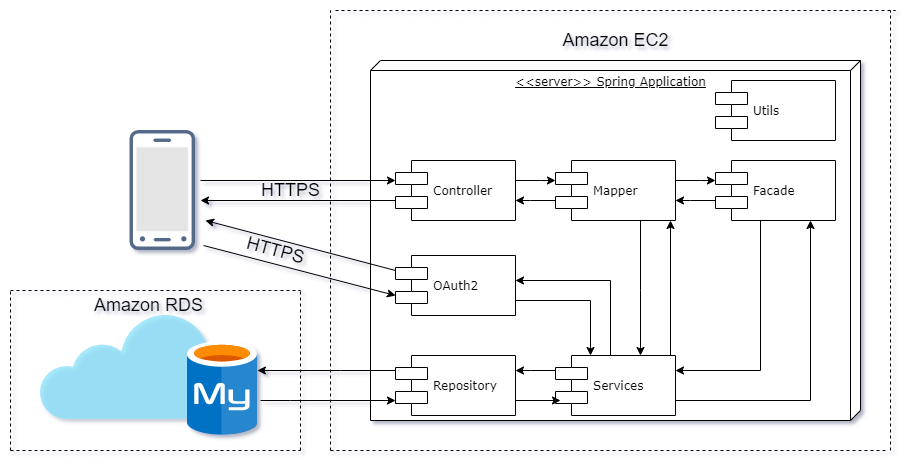
\includegraphics[scale=0.5]{diagrama-componentes-arquitetura}
  \legend{Fonte: Os autores}
\end{figure}

O cliente, que é uma aplicação mobile para Android, realizará requisições ao backend e, assim, conseguir operar suas funcionalidades e exibir os dados no layout de modo coerente no aplicativo.

O servidor, por sua vez, será dividida em camadas lógicas. A camada que será exposta e acessível para o frontend são os endpoints dos controllers, recebendo e retornando DTOs (padrão Data Transfer Object) em formato JSON. Após acessar o endpoint, caso esteja devidamente autenticado no OAuth2 e com o token de autorização, será chamado o mapper, responsável por converter DTO em model.

Após essa conversão, dependendo da complexidade da regra de negócio, pode chamar o service - para regras de negócios simple -  ou um facade - responsável por encapsular regras de negócios complexas, chamando os services a fim de evitar injeção de dependência cruzada entre os services. 

Os services, por sua vez, encapsulam as operações de CRUD do hibernate que são definidas nas Repositories.

Após a realização da requisição, será enviada uma resposta para o frontend, onde o mapper, dessa vez, irá converter o model em DTO, de modo que consiga tratar o dado a partir de formatações, retirada de dados sensíveis e garantindo maior performance ao enviar apenas os dados que serão devidamente utilizados (e não dados em excesso), garantindo menor dados em tráfego na rede, menor consumo de internet e maior velocidade.

O OAuth2 é o serviço de autenticação e autorização adotado que irá se aproveitar dos services para realizar a verificação das credenciais fornecidas no momento do login.

O Utils é uma biblioteca global que pode ser reutilizado em todo o projeto como, por exemplo, validação de dados, formatação de dados, entre outros.

O backend será hospedado no Amazon EC2 e o banco de dados MySQL estará disponível no Amazon RDS.

\subsection{Serviços de Apoio}

No Lixt, haverá serviços de apoio que auxiliarão a cumprir as regras de negócios. 

O primeiro serviço é o de autenticação e autorização, no qual será utilizado o OAuth2 para cumprir essa função. O OAuth2 garante a maior segurança, conseguindo permitir a utilização do sistema a partir do token que foi previamente registrado no sistema (impedindo a criação de token manualmente para acessar a plataforma). Para a autorização do usuário, será solicitado um bearer token. Além disso, garante a escalabilidade, visto que permite a autenticação de outras APIs a partir da geração o próprio token com as credenciais de clientID e secretID - gerando um basic token -, facilitando a integração entre APIs. Inclusive, para um uusário se autenticar com OAuth2, é necessário que o serviço que enviará a requisição possua seu próprio basic token, reforçando a segurança ao garantir que o sistema não estará disponível para ser acessado facilmente.

O segundo serviço é o de email, que será implementado com javamail. Para esse serviço, será criada uma conta de gmail com as configurações habilitadas para enviar email de terceiros (ou seja, da nossa API).
